\documentclass{revtex4}
\usepackage[margin=1in, paperheight=1in, paperwidth=1in]{geometry}  % doesn't compile w/o width, height
\geometry{
 a4paper,
 total={170mm,257mm},
 left=15mm,
 top=5mm,
}
\usepackage{amsmath}
\usepackage{amssymb}
\usepackage{kbordermatrix}
\usepackage{braket}
\usepackage{xcolor}
\usepackage{graphicx}
\usepackage{verbatim}

%\definecolor{myred}{HTML}{990000}
%\definecolor{myblue}{HTML}{002299}
\definecolor{myred}{HTML}{000000}
\definecolor{myblue}{HTML}{000000}

\newcommand{\Ap}{\textcolor{myred}{\left(aj|ib\right)}}
\newcommand{\App}{\textcolor{myred}{\left(aj|bi\right)}}
\newcommand{\Aa}{\textcolor{myred}{\left(aj||ib\right)}}
\newcommand{\B}{\textcolor{myblue}{\left(ab|ij\right)}}
\newcommand{\Br}{\textcolor{myblue}{\left(ab|ji\right)}}
\newcommand{\Ba}{\textcolor{myblue}{\left(ab||ij\right)}}

\newcommand{\AtoB}{\mathbf{\alpha\rightarrow\beta}}
\newcommand{\BtoA}{\mathbf{\beta\rightarrow\alpha}}
\newcommand{\AtoA}{\mathbf{\alpha\rightarrow\alpha}}
\newcommand{\BtoB}{\mathbf{\beta\rightarrow\beta}}
\newcommand{\e}{\textcolor{myred}{\left(\epsilon_a-\epsilon_i\right)}}
\newcommand{\diag}{\textcolor{myred}{\delta_{ij}\delta_{ab}}}


\begin{document}
\title{Notes on Matrix Factorization for Hartree-Fock Stability of HEG}
%\author{Evan Curtin}
\maketitle

\section{Definitions}
According to Seeger and Pople\cite{Seeger1977}, (and many other sources) the molecular orbital
Hessian has the form,
\begin{eqnarray}\label{basic}
\mathbf{H} =
  \begin{bmatrix}
    \mathbf{A}   & \mathbf{B}   \\
    \mathbf{B^*} & \mathbf{A^*} \\
  \end{bmatrix}
\end{eqnarray}
Where the matrices denoted by $\mathbf{A}$ and $\mathbf{B}$ are given by,
\begin{eqnarray}
  A_{st} &=& \e\diag +  \textcolor{myred}{\braket{aj||ib}} \\
  B_{st} &=& \textcolor{myblue}{\braket{ab||ij}}         
\end{eqnarray}
and the two electron integral used here is defined as, 
\begin{eqnarray}
  \braket{pq|rs} &=& \int\int \chi^*_p(1) \chi^*_q(2) \frac{1}{r_{12}} \chi_r(1) 
  \chi_s(2)
  d\tau d\sigma \\
  \braket{pq||rs} &=& \braket{pq|rs} - \braket{pq|sr} \\
  (pq|rs) &=& \int\int \chi^*_p(1) \chi^*_q(2) \frac{1}{r_{12}} \chi_r(1) 
  \chi_s(2)
  d\tau \\
  (pq||rs) &=& (pq|rs) - (pq|sr)
\end{eqnarray}
Where $\sigma$ is the spin coordinate and $d\tau$ is the volume element in all spatial coordinates.
Additionally, the convention of $a, b$ being virtual states, $i, j$ being occupied states and 
$p, q, r, s$ being any state is followed.  

The solution is said to be unstable when the lowest eigenvalue of $\mathbf{H}$
is strictly negative. The
corresponding eigenvector points downhill in energy in the case of instability. Defining
the eigenvector as $\mathbf{D}$, the eigenvalue problem can be written as
\begin{eqnarray}
  \mathbf{HD = \lambda D}
\end{eqnarray}

\section{Transforming H Dictates the form of D}
In many cases, the matrix $\mathbf{H}$ factorizes into various components. The following
form of a similarity transformed eigenvalue problem is useful to keep in mind:
\begin{eqnarray}
  \mathbf{S^{-1} H S S^{-1} D} &=& \mathbf{\lambda S^{-1} D} \\
  \mathbf{\tilde H \tilde D} &=& \mathbf{\lambda \tilde D}   
\end{eqnarray} 

Thus if the matrix $\mathbf{H}$ can be transformed via a similarity transformation defined
by $\mathbf{S}$ into $\mathbf{\tilde H}$, then the corresponding eigenvector which satisfies the 
eigenvalue problem
has the form $\mathbf{\tilde D} = \mathbf{S^{-1}D}$.

This approach is commonly used in the paper to transform into the basis that separates
the real and complex contributions of the eigenvectors when $\mathbf{A}$ and $\mathbf{B}$ are real.
Writing the eigenvalue problem in the form of Seeger \& Pople (eq. 18 in \cite{Seeger1977}), 
we get
\begin{eqnarray}
  \begin{bmatrix}
    \mathbf{A} & \mathbf{B} \\
    \mathbf{B^*} & \mathbf{A^*} 
  \end{bmatrix}
  \begin{bmatrix}
    \mathbf{d} \\
    \mathbf{d^*} 
  \end{bmatrix}
  = 2E_2
  \begin{bmatrix}
    \mathbf{d} \\
    \mathbf{d^*} 
  \end{bmatrix}
\end{eqnarray}
We can now apply the similarity transform defined by the Unitary matrix 
\begin{eqnarray}
  \mathbf{U} = \frac{1}{\sqrt{2}}
  \begin{bmatrix}
    \mathbf{I} & -\mathbf{I} \\
    \mathbf{I} & \mathbf{I} 
  \end{bmatrix}
\end{eqnarray}
after which the transformed eigenvalue problem has the form
\begin{eqnarray}
  \frac{1}{2}
  \begin{bmatrix}
    \mathbf{A + B + A^* + B^*} & \mathbf{-A + A^* + B - B^*} \\
    \mathbf{-A + A^* - B + B^*} & \mathbf{A^* + A - B - B^*} 
  \end{bmatrix}
  \begin{bmatrix}
    \mathbf{d + d^*} \\
    \mathbf{d - d^*} 
  \end{bmatrix}
  &=& 2E_2
  \begin{bmatrix}
    \mathbf{d + d^*} \\
    \mathbf{-d + d^*} 
  \end{bmatrix} \\
  &=& 2E_2
  \begin{bmatrix}
    \mathbf{Re(d)} \\
    \mathbf{Im(d)} 
  \end{bmatrix}
\end{eqnarray}
If $\mathbf{A}$ and $\mathbf{B}$ are both real, $\mathbf{A = A^*}$ and $\mathbf{B = B^*}$ and the 
above simplifies to 
\begin{eqnarray}
  \begin{bmatrix}
    \mathbf{A + B} & \mathbf{0} \\
    \mathbf{0} & \mathbf{A - B} 
  \end{bmatrix}
  \begin{bmatrix}
    \mathbf{Re(d)} \\
    \mathbf{Im(d)} 
  \end{bmatrix}
  &=& 2E_2   
  \begin{bmatrix}
    \mathbf{Re(d)} \\
    \mathbf{Im(d)} 
  \end{bmatrix}
\end{eqnarray}
Clearly, the matrix factorizes into $\mathbf{A+B}$ and $\mathbf{A-B}$. The eigenvectors factorize
into the real and imaginary displacements of the orbitals, respectively. This is equivalent to the 
condition derived in and around eq. 20 in Seeger/Pople for internal and external instabilities of 
real
GHF solutions \cite{Seeger1977}, however this approach applies to any matrix with the same
form as equation \ref{basic}.

\section{Forms of equations with UHF Solution}
In the case of a stationary UHF solution, the elements of matrices $\mathbf{A}$ and $\mathbf{B}$ 
have the following forms, after integrating over spin:
\begin{eqnarray}
  A_{i \rightarrow a, j \rightarrow b} &=& \e\diag \textcolor{myred}{+ 
  \delta_{\sigma_i\sigma_a}\delta_{\sigma_j\sigma_b}\Ap
                     - \delta_{\sigma_a\sigma_b}\delta_{\sigma_i\sigma_j}\App} \\
  B_{i \rightarrow a,j \rightarrow b} &=& 
  \textcolor{myblue}{\delta_{\sigma_a\sigma_i}\delta_{\sigma_b\sigma_j}\B 
             - \delta_{\sigma_a\sigma_j}\delta_{\sigma_b\sigma_i}\Br} 
\end{eqnarray}
Writing down the matrices, where the row index corresponds to $i \rightarrow a$ excitations  and 
the column index corresponds to $j \rightarrow b$ excitations:
\begin{eqnarray*}
  \mathbf{A}&=&\kbordermatrix{
        & \AtoA           & \AtoB           & \BtoA          & \BtoB          \\
  \AtoA & \e\diag + \Aa   & 0               & 0              & \Ap            \\
  \AtoB & 0               & \e\diag - \App  & 0              & 0              \\
  \BtoA & 0               & 0               & \e\diag - \App & 0              \\
  \BtoB & \Ap             & 0               & 0              & \e\diag + \Aa  
}
\end{eqnarray*}
\begin{eqnarray*}
  \mathbf{B}&=&\kbordermatrix{
        & \AtoA           & \AtoB           & \BtoA          & \BtoB          \\
  \AtoA & \Ba             & 0               & 0              & \B             \\
  \AtoB & 0               & 0               & -\Br           & 0              \\
  \BtoA & 0               & -\Br            & 0              & 0              \\
  \BtoB & \B              & 0               & 0              & \Ba            
}
\end{eqnarray*}
\\
These matrices factorize into ``spin conserved'' $(\mathbf{A', B'})$ and
``spin-unconserved'' $(\mathbf{A'', B''})$ parts, to use the language of Seeger
and Pople. Similarly, $\mathbf{H}$ factorizes, with no approximations, into
$\mathbf{H}'$ and $ \mathbf{H}''$
\begin{eqnarray}
\mathbf{H}' =
  \begin{bmatrix}
    \mathbf{A}'   & \mathbf{B}'   \\
    \mathbf{B}'^* & \mathbf{A}'^* \\
  \end{bmatrix}
\end{eqnarray}
\begin{eqnarray}
\mathbf{H}'' =
  \begin{bmatrix}
    \mathbf{A}''   & \mathbf{B}''   \\
    \mathbf{B}''^* & \mathbf{A}''^* \\
  \end{bmatrix}
\end{eqnarray}
The spin conserved matrices are given by

\begin{eqnarray}
  \mathbf{A'}&=&\kbordermatrix{
        & \AtoA           & \BtoB          \\
  \AtoA & \e\diag + \Aa   & \Ap            \\
  \BtoB & \Ap             & \e\diag + \Aa  \\
}
\end{eqnarray}
\begin{eqnarray}
  \mathbf{B'}&=&\kbordermatrix{
        & \AtoA           & \BtoB          \\
  \AtoA & \Ba             & \B             \\
  \BtoB & \B              & \Ba            \\
}
\end{eqnarray}
\\
while the spin-unconserved matrices are given by:
\begin{eqnarray}
  \mathbf{A''}&=&\kbordermatrix{
        & \AtoB           & \BtoA          \\
  \AtoB & \e\diag - \App  & 0              \\
  \BtoA & 0               & \e\diag - \App \\
}
\end{eqnarray}

\begin{eqnarray}
  \mathbf{B''}&=&\kbordermatrix{
        & \AtoB           & \BtoA  \\
  \AtoB & 0               & -\Br   \\
  \BtoA & -\Br            & 0      \\
}
\end{eqnarray}
\\
Thus the spin conserved molecular orbital hessian, is given by
\begin{eqnarray*}
  \mathbf{H'}&=&\kbordermatrix{
        & \AtoA             & \BtoB            & \AtoA             & \BtoB            \\
  \AtoA & \e\diag + \Aa     & \Ap              & \Ba               & \B               \\
  \BtoB & \Ap               & \e\diag + \Aa    & \B                & \Ba              \\
  \AtoA & \Ba^*             & \B^*             & \e\diag + \Aa^*   & \Ap^*            \\
  \BtoB & \B^*              & \Ba^*            & \Ap^*             & \e\diag + \Aa^*  \\
}
\end{eqnarray*}
\\
and the spin unconserved molecular orbital hessian, is given by:
\begin{eqnarray*}
  \mathbf{H''}&=&\kbordermatrix{
        & \AtoB           & \BtoA              & \AtoB             & \BtoA            \\
  \AtoB & \e\diag - \App  & 0                  & 0                 & -\Br             \\
  \BtoA & 0               & \e\diag - \App     & -\Br              & 0                \\
  \AtoB & 0                 & -\Br^*           & \e\diag - \App^*  & 0                \\
  \BtoA & -\Br^*            & 0                & 0                 & \e\diag - \App^* \\
}
\end{eqnarray*}

The eigenvalue equation defining $\mathbf{D}'$ is, 
\begin{eqnarray}\label{hppeval}
  \mathbf{H'D'} = 
  \mathbf{H'}
  \begin{bmatrix}
    \mathbf{d_\AtoA} \\
    \mathbf{d_\BtoB} \\
    \mathbf{d^*_\AtoA} \\        
    \mathbf{d^*_\BtoB} 
  \end{bmatrix}
  = 2E_2
  \begin{bmatrix}
    \mathbf{d_\AtoA} \\
    \mathbf{d_\BtoB} \\
    \mathbf{d^*_\AtoA} \\        
    \mathbf{d^*_\BtoB} 
  \end{bmatrix}
\end{eqnarray}

Applying the transformation defined by the unitary matrix, 
\begin{eqnarray}
  \mathbf{U} = \frac{1}{\sqrt{2}} 
  \begin{bmatrix}
    \mathbf{1} & -\mathbf{1} & 0 &  0 \\
    \mathbf{1} &  \mathbf{1} & 0 &  0 \\
    0 &  0 & \mathbf{1} & -\mathbf{1} \\
    0 &  0 & \mathbf{1} &  \mathbf{1} \\
  \end{bmatrix}
\end{eqnarray}

With no further assumptions, this transformation doesn't do much. However, if the spatial
orbitals corresponding to $\alpha$ and $\beta$ are assumed equivalent, the 
transformed $\mathbf{H}'$ is
\begin{eqnarray*}
  \hspace{-1cm}
  \mathbf{U^{-1}H'U} =
  \begin{bmatrix}
    \e + \Aa + \Ap & 0              & \Ba + \B            & 0            \\
    0                    & \e + \Aa - \Ap    & 0                & \Ba - \B              \\
    \Ba^* + \B^*         & 0                & \e+ \Aa^* + \Ap^*   & 0                     \\
    0                    & \Ba^* - \B^*     & 0                 & \e+ \Aa^* - \Ap^*  \\
  \end{bmatrix}
\end{eqnarray*}

while the corresponding eigenvectors are 
\begin{eqnarray*}
  \mathbf{U^{-1}D'} = \frac{1}{\sqrt{2}}
  \begin{bmatrix}
    \mathbf{d_\AtoA + d_\BtoB} \\
    \mathbf{d_\AtoA - d_\BtoB} \\
    \mathbf{d^*_\AtoA + d^*_\BtoB} \\        
    \mathbf{d^*_\AtoA - d^*_\BtoB} 
  \end{bmatrix}
\end{eqnarray*}

In this basis the equations clearly factorize into the following sets of eigenvalue equations:  
\begin{eqnarray}\label{1Heval}
  \begin{bmatrix}
    \e + \Aa + \Ap & \Ba + \B          \\
    \Ba^* + \B^*   & \e+ \Aa^* + \Ap^* \\
  \end{bmatrix}
  \begin{bmatrix}
    \mathbf{d_\AtoA + d_\BtoB} \\
    \mathbf{d^*_\AtoA + d^*_\BtoB} \\        
  \end{bmatrix}
  = 2E_2
  \begin{bmatrix}
    \mathbf{d_\AtoA + d_\BtoB} \\
    \mathbf{d^*_\AtoA + d^*_\BtoB} \\        
  \end{bmatrix}
  \vspace{5mm}
  \\ \label{3Heval}
  \begin{bmatrix}
    \e + \Aa - \Ap & \Ba - \B          \\
    \Ba^* - \B^*   & \e+ \Aa^* - \Ap^* \\
  \end{bmatrix}
  \begin{bmatrix}
    \mathbf{d_\AtoA - d_\BtoB} \\
    \mathbf{d^*_\AtoA - d^*_\BtoB} \\        
  \end{bmatrix}
  = 2E_2
  \begin{bmatrix}
    \mathbf{d_\AtoA - d_\BtoB} \\
    \mathbf{d^*_\AtoA - d^*_\BtoB} \\        
  \end{bmatrix}
\end{eqnarray}
Equation \ref{3Heval} defines the matrix ${{}^3\mathbf{H}'}$, the triplet instability matrix,
while \ref{1Heval} defines the matrix ${{}^1\mathbf{H}'}$, which defines instabilities that mix 
singlet states. The only assumption made until this point in the analysis of ${\mathbf{H}'}$ was
that the original solution was a complex RHF solution. No assumption was made about the outside 
space towards which the eigenvector points. Even still, the eigenvectors can be shown to have the
form given in equations \ref{1Heval} and \ref{3Heval}. Thus, the space in which the eigenvectors
of ${\mathbf{H}'}$ point can only be that of UHF solutions. 

Now, the other part of the general form of the stability matrix is ${\mathbf{H}''}$.
The eigenvalue equation defining $\mathbf{D}''$ is, 
\begin{eqnarray}\label{hppeval}
  \mathbf{H''D''} = 
  \mathbf{H''}
  \begin{bmatrix}
    \mathbf{d_\AtoB} \\
    \mathbf{d_\BtoA} \\
    \mathbf{d^*_\AtoB} \\        
    \mathbf{d^*_\BtoA} 
  \end{bmatrix}
  = 2E_2
  \begin{bmatrix}
    \mathbf{d_\AtoB} \\
    \mathbf{d_\BtoA} \\
    \mathbf{d^*_\AtoB} \\        
    \mathbf{d^*_\BtoA} 
  \end{bmatrix}
\end{eqnarray}

Equation \ref{hppeval} clearly factors into the following two eigenvalue equations:
\begin{eqnarray}\label{b2aa2b}
    \kbordermatrix{
          & \BtoA              & \AtoB            \\
    \BtoA & \e\diag - \App     & -\Br             \\
    \AtoB & -\Br^*           & \e\diag - \App^* \\
  }
  \begin{bmatrix}
    \mathbf{d_\BtoA} \\
    \mathbf{d^*_\AtoB} \\        
  \end{bmatrix} 
  &=& 2E_2
  \begin{bmatrix}
    \mathbf{d_\BtoA} \\
    \mathbf{d^*_\AtoB} \\        
  \end{bmatrix}
  \\
  \label{a2bb2a}
    \kbordermatrix{
          & \AtoB              & \BtoA            \\
    \AtoB & \e\diag - \App     & -\Br             \\
    \BtoA & -\Br^*           & \e\diag - \App^* \\
  }
  \begin{bmatrix}
    \mathbf{d_\AtoB} \\
    \mathbf{d^*_\BtoA} \\        
  \end{bmatrix} 
  &=& 2E_2
  \begin{bmatrix}
    \mathbf{d_\AtoB} \\
    \mathbf{d^*_\BtoA} \\        
  \end{bmatrix}
\end{eqnarray}

Equations \ref{b2aa2b} and \ref{a2bb2a} are complex conjugates in the general case. If however, 
the solution is an RHF solution, the spatial orbitals for $\alpha$ and $\beta$ spins are identical
by definition. In this case, the matrices in both equation \ref{b2aa2b} and equation \ref{a2bb2a}
are equivalent to the triplet instability matrix defined by Seeger and Pople:

\begin{eqnarray}
  \mathbf{{}^3H} =
  \begin{bmatrix}
    \e \diag - (aj|bi) & -(ab | ji )           \\
    -(ab | ji )^*        & \e \diag - (aj|bi)^* \\        
  \end{bmatrix} 
\end{eqnarray}

The implication of equations \ref{b2aa2b}, \ref{a2bb2a} and \ref{3Heval} is that the following 
sets of eigenvectors comprise a degenerate manifold when the solution is an RHF wavefunction.
\begin{eqnarray}
  \begin{bmatrix}
    \mathbf{d_\BtoA} \\
    \mathbf{d^*_\AtoB} \\        
  \end{bmatrix}
  , 
  \begin{bmatrix}
    \mathbf{d_\AtoB} \\
    \mathbf{d^*_\BtoA} \\        
  \end{bmatrix}
  ,
  \begin{bmatrix}
    \mathbf{d_\AtoA - d_\BtoB} \\
    \mathbf{d^*_\AtoA - d^*_\BtoB} \\        
  \end{bmatrix}
\end{eqnarray}
As such, the RHF-GHF instability eigenvectors can always be transformed into eigenvectors having the
form of the RHF-UHF instability. On the other hand, if the solution is not an RHF solution, this is
not the case and the eigenvalues/vectors and corresponding instabilities are distinct.  

\section{Numerical result}
To verify numerically, the diagonalization of the matrices $\mathbf{H}, \mathbf{H}'$ and 
${}^3\mathbf{H}'$ were implemented independently of one another. No factorizations or 
simplifications were performed. The lowest eigenvalue of each is shown below for a constant number
of K-points and a varying density. The results are equivalent within the convergence criteria of 
Davidson's Algorithm.  
\begin{figure}[h]
  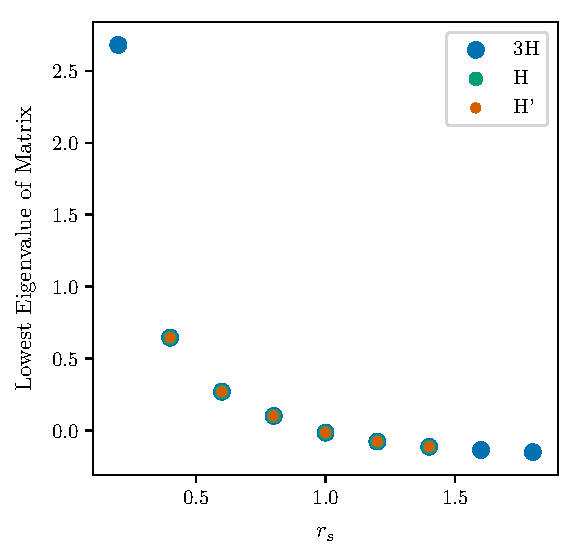
\includegraphics[width=0.75\linewidth]{../../images/Matrix_Compare.pdf}
\end{figure}

\begin{comment}
\section{Proof of Real-Valued A and B}
In the case of the Homogeneous electron gas,
the two electron integral is given by
(eq. 12 of~\cite{Delyon2008} and p. 16 of~\cite{Guiliani2005}):

\begin{subequations}
\begin{align}
\braket{\vec{k}, \vec{k}'|\vec{k}'',\vec{k} '''}\stackrel{\text{2D, 3D}}{=}&
	\begin{cases}
	\frac{\pi}{\Omega}\frac{2^{D-1}}{|\vec{k}-\vec{k}''|^{D-1}}
	& \vec{k}''' = \vec{k}+\vec{k}'-\vec{k}'' \textbf{ and } |\vec{k}-\vec{k}''| \neq 0 \\
	0
	& \text{else}
	\end{cases}
\\ \nonumber \\
\braket{k, k'|k'',k'''}\stackrel{\text{1D}}{=}&
	\begin{cases}
	e^{|k-k''|^2a^2}\text{Ei}(-|k-k''|^2a^2)\text{;}
	& k''' = k + k'-k'' \textbf{ and } |k-k''| \neq 0 \\
	0\text{;}
	& \text{else}
	\end{cases}
\end{align}
\end{subequations}

The two electron integrals are always real-valued. Therefore
$\mathbf{A} = \mathbf{A}^*$ and $\mathbf{B} = \mathbf{B}^*$

So far I have not used this to simplify anything, but it is true.
\end{comment}
\section{References}
\bibliography{../heg_references}
\end{document}
